\tightsection{Implementation and Scalability}
\label{sec:impl}

In this section, we present the high level GO implementation. While there are much details in building GO system, we focus on the two main components: data processing and decision making. Paramount in our implementation was the need to make very rapid decisions, as any extra delay in decision making could impact performance of the client making the request. This meant that the vast majority of prediction information needed to be precomputed. This resulted in an implementation that involves two parts: computation and updating of a group table every minute, and broadcasting of said table out to servers close to the clients making requests.

%The GO backend collects information (including quality samples) sent back by clients, processes the information periodically to aggregate the information, and then, upon on receiving a request from a new session, the best decision can be made quickly.

%Like many data processing systems, individual events from every single client sending information must be rolled up and summarized into a succinct format. Because many systems do this, and there is nothing specific to our problem about how this is done, we will focus on how the system rapidly translates these summaries into meaningful pieces of information used for prediction and decision making. These summaries consist of the most recent performance information about a session, as well as the information about what decision was made for the session. 

\myparatight{Creating group table} Group table generation is essentially the process of aggregating samples into buckets, and then computing summary statistics for each bucket.  
Our implementation uses Spark~\cite{} as the underlying compute framework, and the problem can be captured in a single map-reduce stage. 
Data samples are loaded in parallel from an HDFS source and distributed amongst the cluster. Each node then maps its share of samples to a set of 
preliminary buckets. Common buckets are then shuffled across the cluster and the results are aggregated and collected onto a master machine. 
Currently it takes GO system 12 seconds to process 500K identical groups on a 4-node cluster, without riguous performance optimization.
It is also worth noting that all steps involved in creating the table are horizontally scalable.

\comment{
\begin{figure}[h!]
\centering
 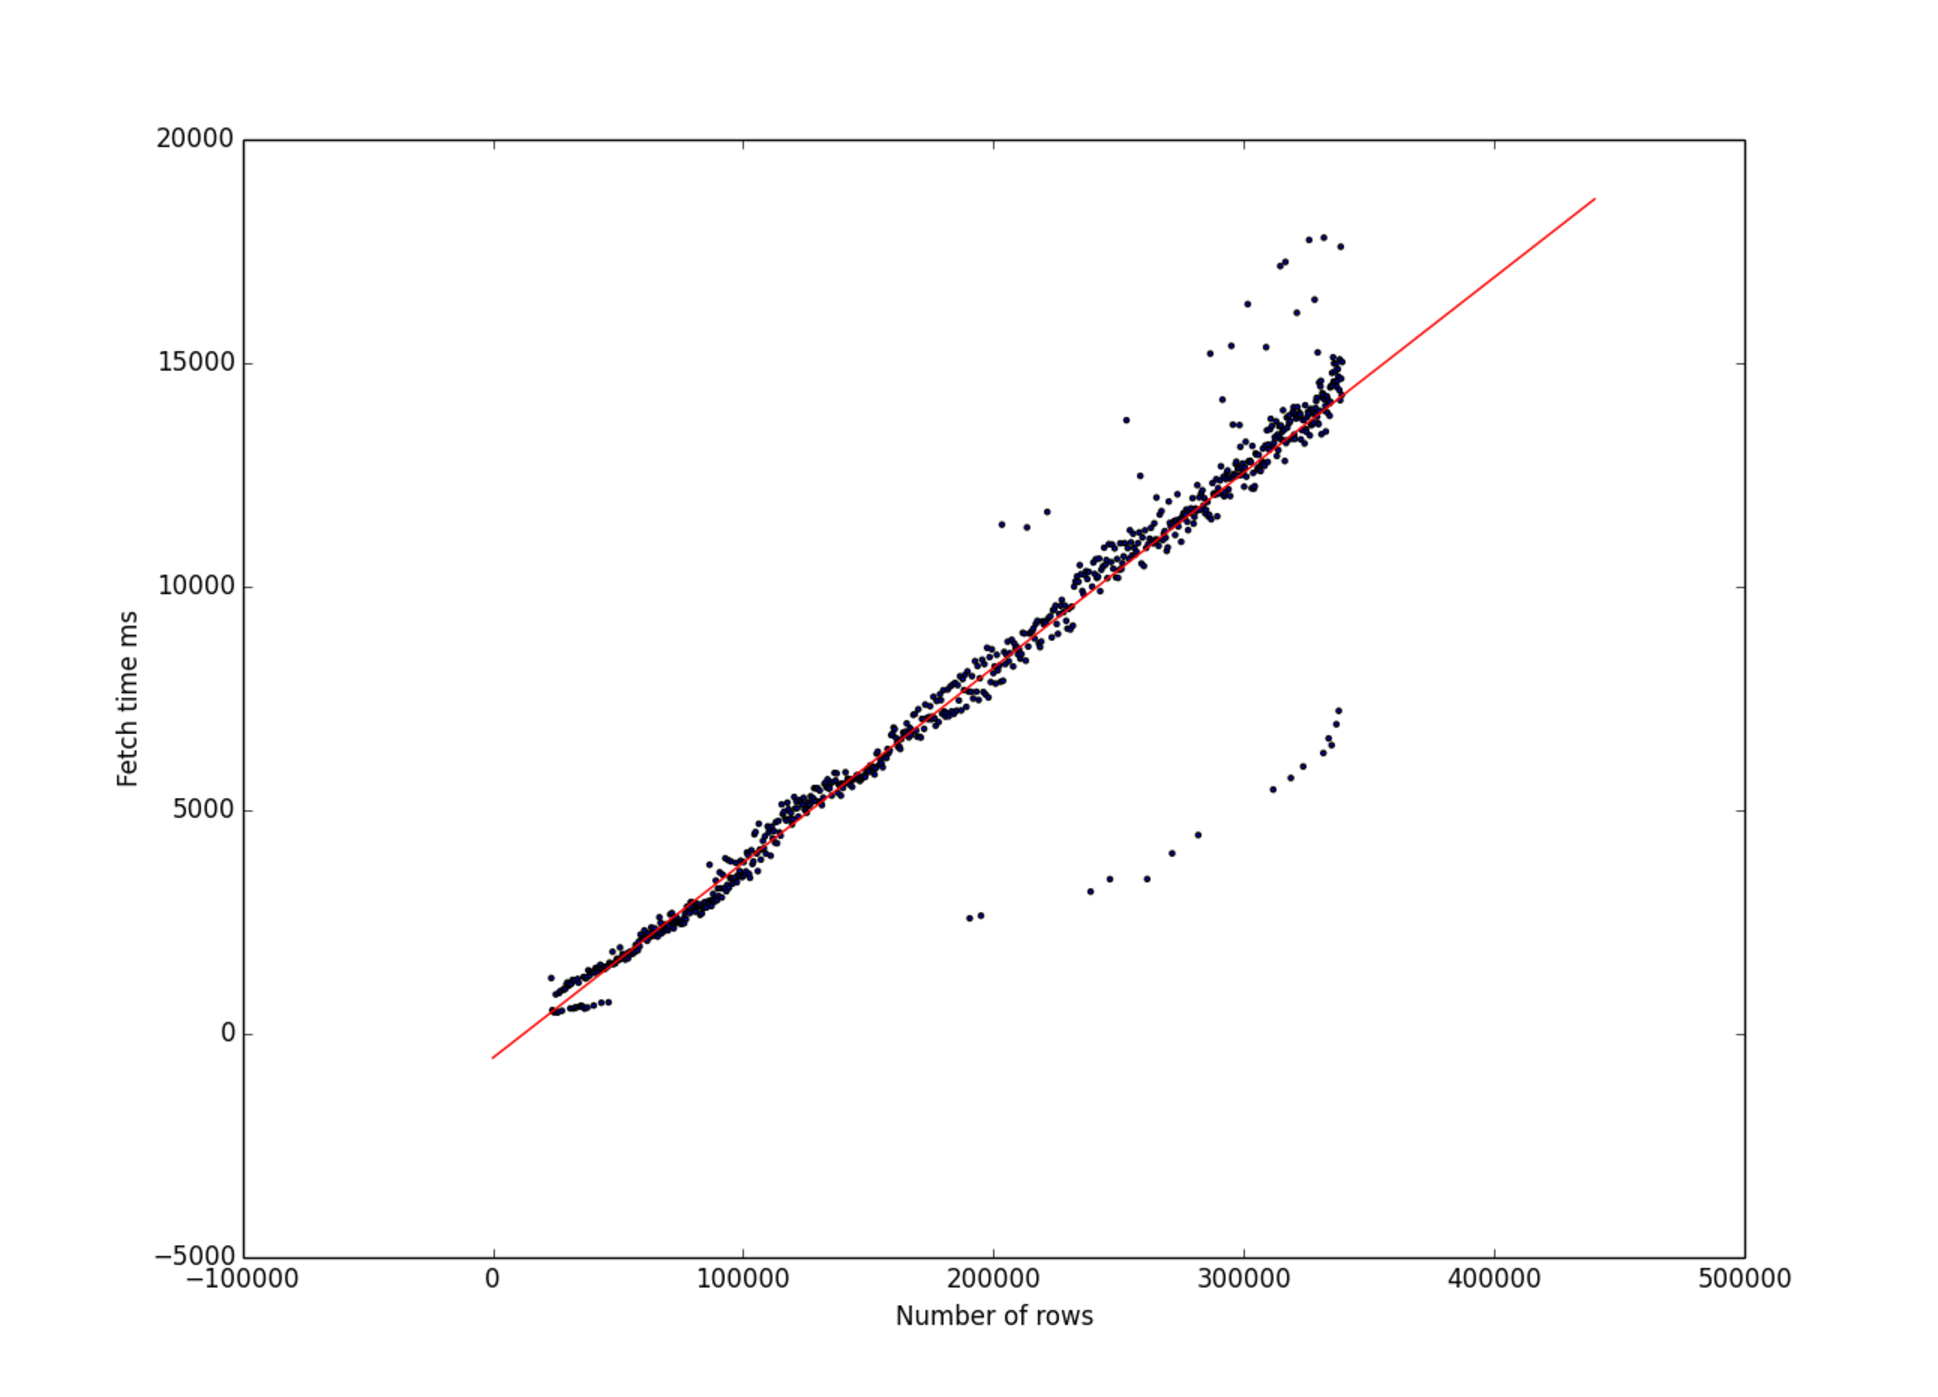
\includegraphics[width=0.5\textwidth] {figures/scale/fetch_time_scale.pdf}
\tightcaption{Dummy figure. This will essentially be overlaid multiple scatter plots from different cluster
sizes to show that increasing cluster size improves computation time}
\label{fig:computing-scale}
\end{figure}
}

\myparatight{Broadcasting group table} The resulting table is broadcasted wholesale out to a large number of decision makers (DMs) closer to video clients in multiple POPs by way of a distributed messaging system~\cite{kafka}. The bottleneck here is bandwidth, because at minimum, we need to ship one table copy to each POP where we deployed decision makers. We believe this is justified by providing quick response to video players. Our current GO table size is 50MB for 500K entries, with an update frequency of one minute, the bandwidth required is 0.83Mbps per POP. We would like to note that we have not optimized serialization and deserialization in terms of size.

\comment{
\begin{figure}[h!]
\centering
 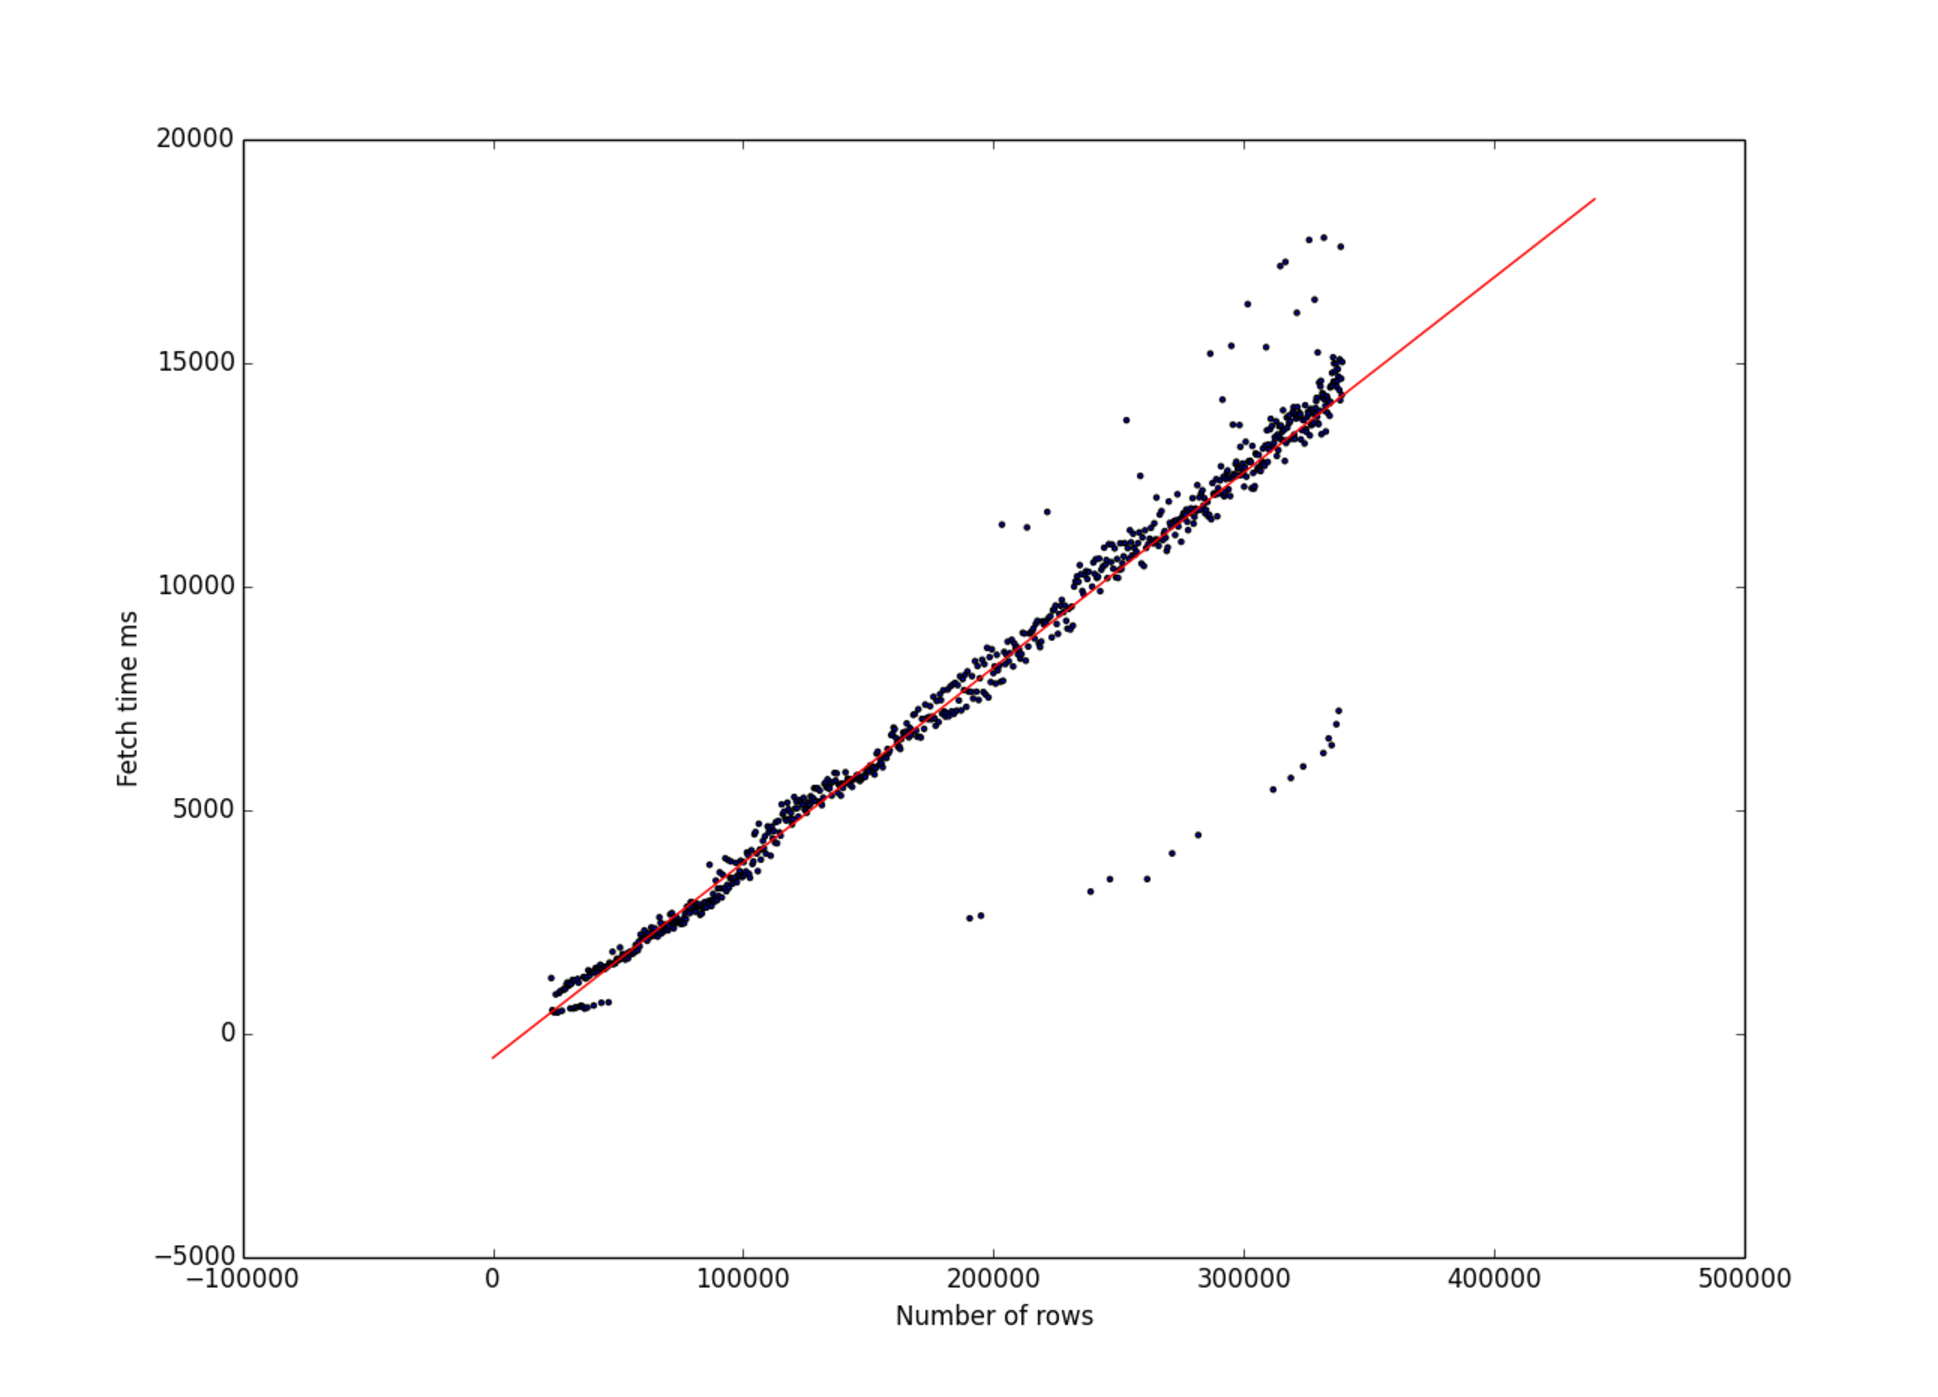
\includegraphics[width=0.5\textwidth] {figures/scale/fetch_time_scale.pdf}
\tightcaption{Time to fetch versus table size.}
\label{fig:fetching-scale}
\end{figure}
}

\myparatight{Decision making} Once a decision maker has a table, decision making is a matter of running the prediction algorithm for evaluation of each decision. Given that there are $N$ ACs for decision evaluation, and $M$ possible decisions, there are $M \times N$ lookups for a decision to be made. The decision making process is horizontally scalable by adding more decision makers, and in general, decision making is extremely fast. The average response time from current GO system is $0.62 ^{+}_{-} 0.016$ms with 3 decision makers (both query per second and CPU utilization are low on the decision makers), which is insignificant compared to RTT in Internet.

% XI: I removed this figure because it does not too much value than just spell out the response time.
\comment{
\begin{figure}[h!]
\centering
 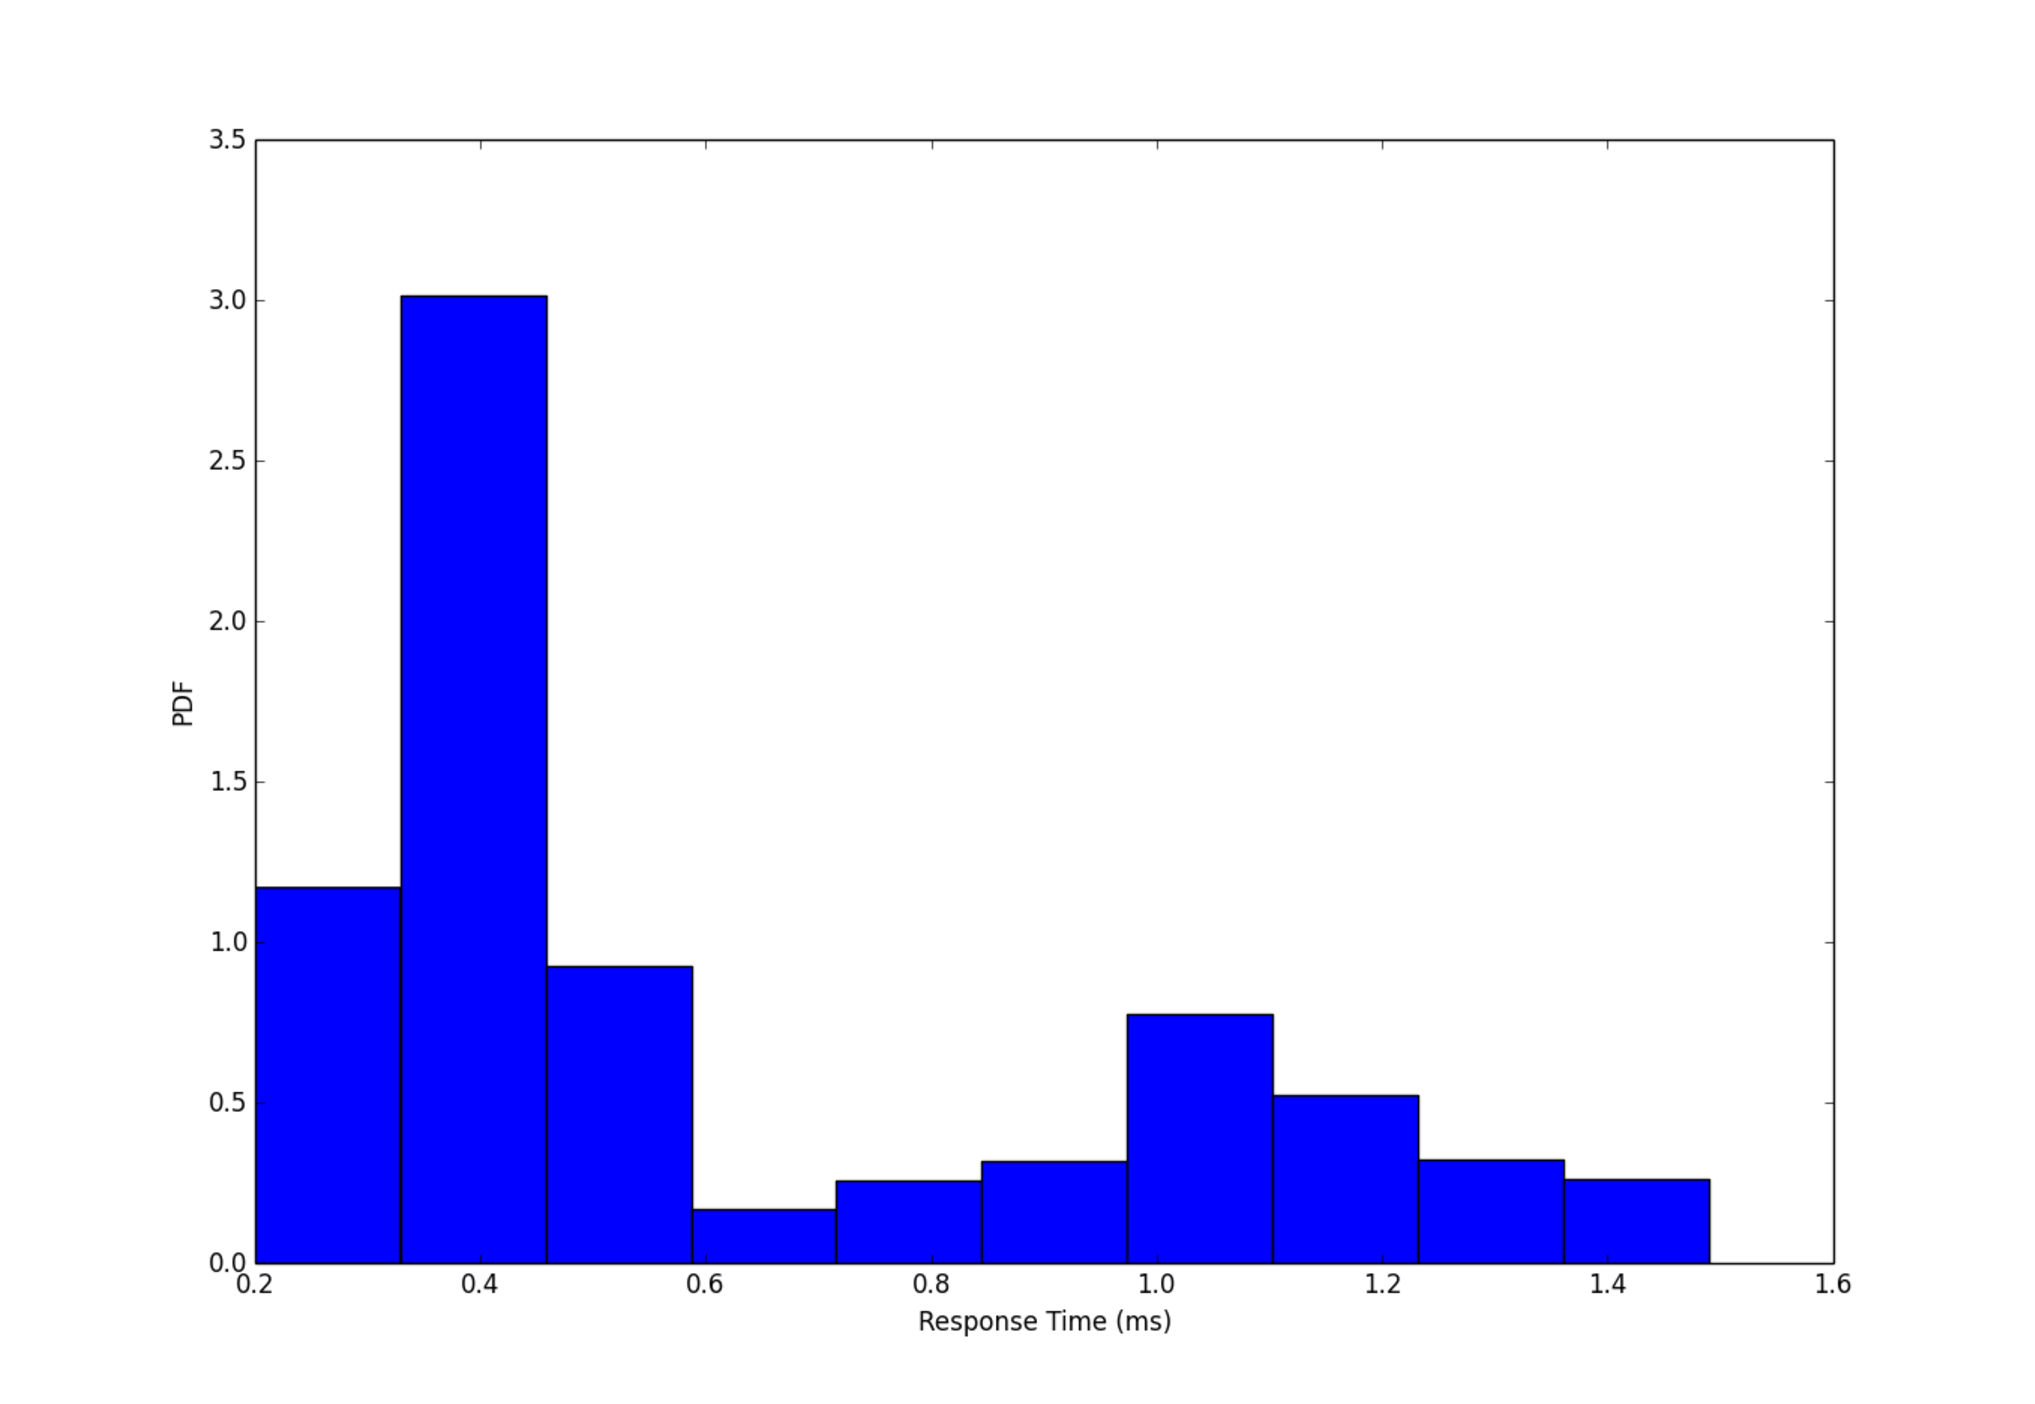
\includegraphics[width=0.5\textwidth] {figures/scale/query_scale.pdf}
\tightcaption{Query times PDF.}
\label{fig:query-scale}
\end{figure}
}

In summary, we implemented GO which is both scalable and provide good system-level performance.

% \tightsection{Scalability}
% The goal of this section is to show that our implementation of the GO backend is scalable for centralized processing, including to continuously collect and process massive client-side measurement and based on the result, make decision for each video session of a large number of viewers. That said, we need to examine 
% \begin{packeditemize}
% \item The general scalability of handling updates and queries of the GO backend, and
% \item The scalability of GO decision making which gets quality samples from quality sample storage and answers query for best decision to querying sessions.
% \end{packeditemize}
% %Note that our implementation leverages several existing techniques (e.g., quality sample aggregation uses Spark). We will also discuss the impact of our particular implementation on the performance.
% 
% \tightsubsection{Backend throughput}
% 
% We need to show that performance (using certain metric) as a function of the number of quality samples (i.e., heartbeats), and the number of session under prediction (i.e., GO precision queries) (and other factors that might impact the scalability of backend throughput). This is to confirm that the backend (excluding GO) is not the bottleneck.
% 
% \tightsubsection{GO scalability}
% 
% The GO implementation has two separate jobs that run in parallel: (1) creating group table -- to fetch the quality samples from quality sample storage, process them into a group table and broadcast the group table to query responders, and (2) decision making -- to answer the query by responders. 
% 
% The delay of creating group table determines the freshness of information based on which the decisions are made. If this step takes $t$ seconds, the decision has to be made based only information that was at least $t$ seconds ago. Delay of decision making is a critical part of the responsiveness of GO backend and potentially a bottleneck of how quickly the client video gets the decision which is very sensitive to video quality when making initial decisions. 
% We should show the performance of both metrics and memory requirement as a function of workload and computational resource as well. 
% \fillme
% 
% 
% 
% 
% \myparatight{Decision making} We then examine the delay of decision making. \fillme

%There are four parts in GO backend that can potentially become performance bottleneck -- user-facing gateway, quality sample storage, quality sample aggregation using ACS, and making individual decisions. To show the scalability, we use micro-benchmark to test their performance as a function of workload (e.g., number of quality samples and queries).


%\tightsection{Quality sample storage}
%Show that quality samples can be processed and stored in an HDFS in parallel. Show runtime as a function number of quality sample updates. \fillme

%\tightsection{Quality sample aggregation}
%Show that quality sample aggregation can be finished in one minute, so that it can be carried every minute. Show both of its running time and memory requirement as a function of number of quality samples and choices of ACS. \fillme

%\tightsection{Making individual decisions}
%Show that once quality samples are aggregated, GO backend can make decsion based on this aggregated information in parallel. Show running time and memory requirement as a function of number of sessions under prediction. \fillme

%\tightsection{User-facing gateway}
%Show that all quality sample updates and queries for best decision will be received and processed immediately. \fillme
